\documentclass{article}

\usepackage{a4wide}
\usepackage{graphicx}
\usepackage{fancybox}
\usepackage{ascmac}
\usepackage{xspace}
\usepackage{pdfpages}
\usepackage{pifont}
\usepackage{array}
\usepackage{multirow}
\usepackage{threeparttable} 
\usepackage{color}
\usepackage{float}

\newcommand\st{\textsuperscript{st}\xspace}
\newcommand\nd{\textsuperscript{nd}\xspace}
\newcommand\rd{\textsuperscript{rd}\xspace}

\begin{document}

% cover letter
\begin{flushleft}
  2016-06-10\newline
  EMSOFT 2016 Submission \#83\newline
  Title: Exploring the Performance of ROS2\newline
  %% Authors: Yuya Maruyama, Shinpei Kato, and Takuya Azumi\newline
\end{flushleft}
\textbf{Dear Reviewers,}\newline

We highly appreciate the insightful suggestions and detailed valuable comments on our paper. The suggestions of the reviewers are very helpful for us and the suggestions are now incorporated in the revised paper as follows. We have attached the last paper review and revised paper in our reply letter. In the revised paper, newly added and modified sentences are written in the bold and red colored font so that the reviewers can easily find them. We hope the reviewers will be satisfied with our replies to the comments and the revised paper.\newline\newline

\begin{flushleft}
  Yours sincerely,\newline
  authors
  %% Yuya Maruyama\newline
  %% Osaka university\newline
  %% Email address: maruyama@hopf.sys.es.osaka-u.ac.jp\newline
\end{flushleft}

\clearpage


% \section{Response to Meta-reviewer}
% \subsection{Recommendations and Relationale for Decision 1}

% \begin{flushleft}
%   \textbf{Comment:}
% \end{flushleft}

% \begin{flushleft}
%   \textbf{Our reply:}
% \end{flushleft}

% \begin{itembox}[|]{hoge }
% \end{itembox}\\

% \begin{itembox}[|]{hoge}
%   $\bullet$\\
%   $\bullet$\\
% \end{itembox}

% \subsection{Recommendations, Retionale for Decision 2}

% \begin{flushleft}
%   \textbf{Comment:}
% \end{flushleft}

% \begin{flushleft}
%   \textbf{Our reply:}
% \end{flushleft}


% \newpage


\section{Response to 1\st reviewer}

\subsection{Premature ROS2 for evaluation}
\begin{itemize}

\item \begin{flushleft}
    \textbf{Comment:}
  \end{flushleft}
  ROS2 is currently still being actively developed (Section 3) and as such, an analysis of the performance at this stage seems a pre-mature. Certain capabilities in ROS2 are still not available and/or do not perform up to expectations. In Section 3.2 the author claims that "DDS is not designed to handle large data", however DDS has API's specifically designed for use with large data packets. While DDS has these API’s for assisting with large packet transfer, they are not yet compatible with ROS2 and therefore the performance drops after the size of packets increases beyond 64KB.

  \begin{flushleft}
    \textbf{Our reply:}
  \end{flushleft}
  Thank you very much for your vital comment.
  It is true that ROS2 in under heavy development and a very rough draft in this statge.
  However, this paper aims to conduct proof of concept for DDS approach to ROS and clarifies the needs of abstracting DDS API for large packets.
  Regardless of development stage of ROS2, we consider that understanding each DDS characteristics is meaningful for ROS2 users, which we provide in this paper.
  After reading your comment, we have highlighted that this paper aims to proof of concept and arranged premature points of current ROS2.
  \begin{itembox}[|]{Modified sentences about proof of concept in ``1. INTRODUCTION'' section}
    \textbf{Contribution:}
    In this paper, we provide proof of concept for DDS approach to ROS.
    We clarify the performance characteristics of the currently available data transport for ROS1 and ROS2 in various situations.
    Focusing on the present capabilities of ROS2, depending on DDS vendor and configuration, we explore and evaluate the potential and constraints from several aspects: latency, throughput, thread, and memory.
    From experimental results, we arrange guidelines for ROS users and what we can do to solve current constrains.
    To the best of our knowledge, this is the first study to explore ROS2 performance.
  \end{itembox}\\
  \begin{itembox}[|]{Added sentences about improvements for current ROS2 in ``Lessons Learned'' section}
    However, ROS2 is under development and there is room to improve its performance and capability.
    First, current \emph{QoS Policies} supposed by ROS2 provide fault tolerance but they are insufficient for real-time processing.
    ROS2 has to expand the scope of supported \emph{QoS Policies}.
    Second, for small embedded system, ROS2 needs minimum DDS implementation and minimum abstraction layer.
    C library for ROS2 and small DDS implementation are needed and ROS2 support them easily.
    Third, we also clarify a need of alternative API for large \emph{message} to manage divided packets.
    This is critical to handle large message.
    Abstraction of this will shorten DDS end-to-end latency and fulfill deficiency of Table \ref{tb:capabilities}.
    Finally, we must tune DDS configurations for ROS2 beacause there are numerous vendor specific configuration options which might affect its performance.
  \end{itembox}\\

\end{itemize}

\subsection{Narrow scope of experiments}
\begin{enumerate}

\item \begin{flushleft}
    \textbf{Comment:}
  \end{flushleft}
  The designed experiment only covers latency rates between the two versions of ROS, but there are still other aspects to communications performance. Further research should be conducted to test the throughput, fault tolerance and distributed capabilities of the two.

  \begin{flushleft}
    \textbf{Our reply:}
  \end{flushleft}
  

\item \begin{flushleft}
    \textbf{Comment:}
  \end{flushleft}
  Interacting with multiple devices or experimentation with a real-time application would provide insight into the fault-tolerance and distributed capabilities that DDS brings to ROS.

  \begin{flushleft}
    \textbf{Our reply:}
  \end{flushleft}
  Thank you for your advice.
  To consider multiple devices, we have conducted evaluations for a multiple destinations publisher.
  Much of the information is often shared in real applications such as robots.
  In our evaluation, we prepare five subscribes and measure end-to-end latencies.
  \begin{itembox}[|]{Added sentences about multiple destination in ``'' section}
  \end{itembox}\\

\item \begin{flushleft}
    \textbf{Comment:}
  \end{flushleft}
  Results from an application would provide insight into how the overhead of DDS scales with increased network load.

  \begin{flushleft}
    \textbf{Our reply:}
  \end{flushleft}


\item \begin{flushleft}
    \textbf{Comment:}
  \end{flushleft}
  Another possible avenue of research is a more detailed analysis of the effects on performance of varying QoS policy variables such as deadline scheduling and history.

  \begin{flushleft}
    \textbf{Our reply:}
  \end{flushleft}
  Thank you for your advice.
  At present, QoS Policy supported by ROS2 is few.
  For example, DEADLINE is only calculated by node's period and is not utilized for scheduling.
  In this condition, we prepare *-depth policy and have varied history setting by configuring depth option.
  This HISTORY QoS Policy provides applications fault tolerance.
  We have added evaluation and its analysis in ``Comparison within ROS2'' section.
  \begin{itembox}[|]{Added sentences in history evaluation in ``Comparison within ROS2'' section}
    Figure \ref{fig:depth_boxplot} shows no differences depending on the depth of \texttt{*-depth policy}.
    These \emph{QoS policies} are different in the number \emph{nodes} save \texttt{messages}.
    Although this number influences resources, this does not affect latency because archiving \emph{messages} is conducted in every publication.
  \end{itembox}\\
  \renewcommand{\arraystretch}{1.0}
  \begin{table}[H]
    \caption{\label{tb:depth_qos}Depth Configurable QoS Policies}
    \centering
    \tabcolsep = 1.5mm              % side-margin in column
    \begin{tabular}{c|c}
      \hline
      & \textbf{\texttt{*-depth policy} }\\
      \hline
      \hline
      DEADLINE & \texttt{100 ms}\\
      HISTORY & \texttt{LAST}\\
      depth & 1, 10, or 100\\
      RELIABILITY & \texttt{RELIABLE}\\
      DURABILITY & \texttt{TRANSIENT\_LOCAL}\\
      \hline
    \end{tabular}
  \end{table}
  \setcounter{figure}{15}
  \begin{figure}[H]
    \centering
    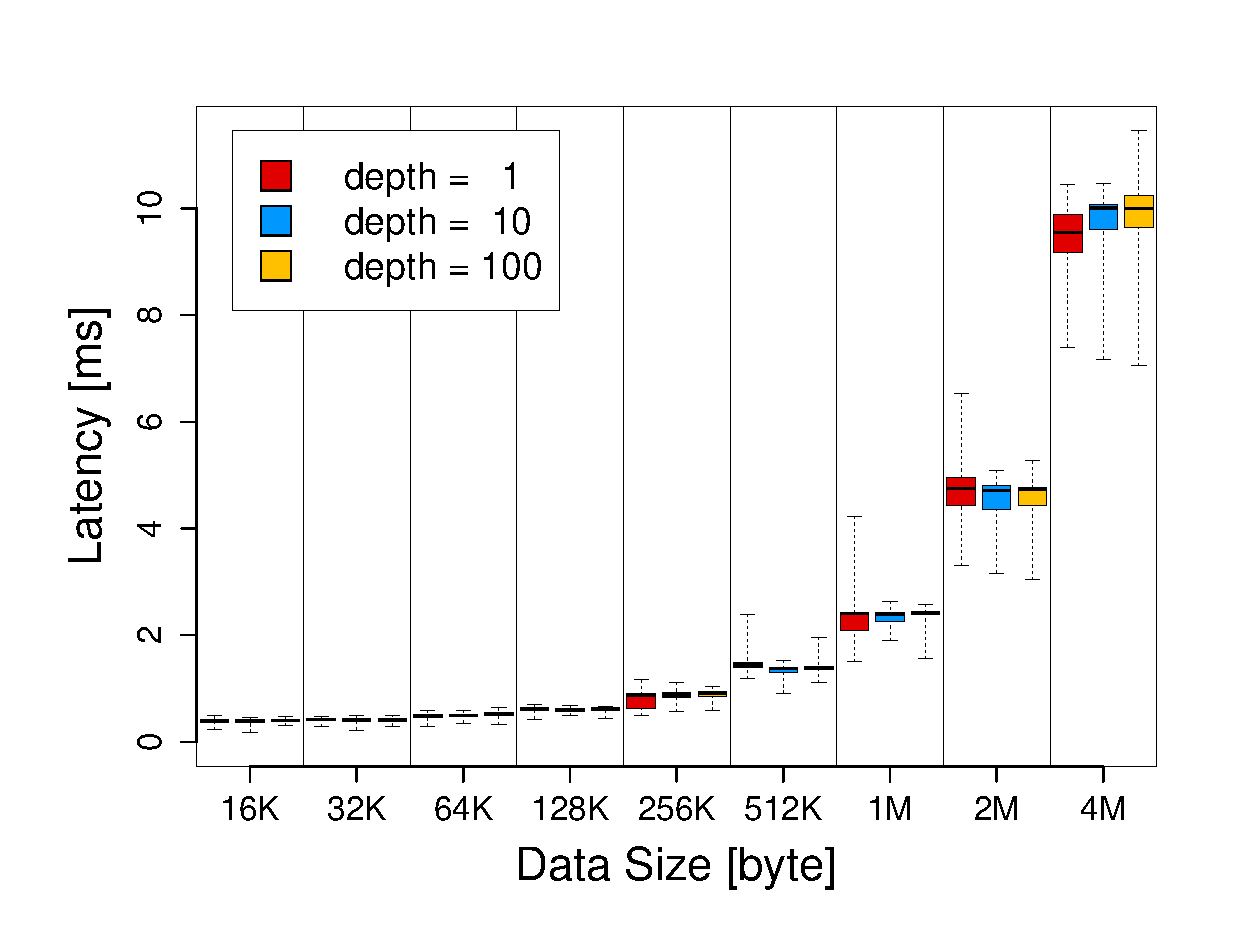
\includegraphics[width=0.6\linewidth]{../../figure/BoxPlot_ospl_QoS_depth.eps}
    \caption{(2-b) Configured \emph{*-depth policy} in ROS2 with OpenSplice}
    \label{fig:depth_boxplot}
  \end{figure}

\item \begin{flushleft}
  \textbf{Comment:}
  \end{flushleft}
  The experiment in section 3.1 should be kept as it is a good evaluation of overhead and is reproducible since it was performed on the loopback interface of the device, but experiments measuring latency and throughput in an application environment would strengthen the paper.

  \begin{flushleft}
    \textbf{Our reply:}
  \end{flushleft}
  Thank you for your thoughtful comment. 
  Following your advice, we additionally conduct a throughout evaluation in Section 3.4.
  Figure 17 clarifies overhead data for DDS transaction.
  Figure 18 shows throughput is limited by the 100 Mbps Ethernet network and not by DDS.
  \begin{itembox}[|]{Added ``3.4 Throughput of ROS1 and ROS2'' section}
    We also measure each throughput of ROS1 and ROS2 in \texttt{remote} case.
    In our one-way message transport experiment, maximum bandwidth ot the network is 12.5MB/sec because we use 100 Mbps Ethernet (100BASE-TX) and Full-Duplex as shown in Table 2.
    Nodes repeatedly transport each data size messages with 10Hz.

    In small data from 256 B to 2 KB, we can observe constant gap among ROS1, ROS2 with OpenSplice, and ROS2 with Connext from Figure 17.
    These additional data correspond with RTPS packets for QoS and heartbeat.
    Hence, these gap does not depend on data size.
    Moreover, Connext throughput is lower than OpenSplice one.
    This becomes significant impact when users handle many kinds of small data with high Hz.

    In large data from 2 KB to 4MB, curves of Figure 18 demonstrate sustainable theoretical throughput.
    ROS2 and ROS2 is able to utilize all of available bandwidth and similarly behave in this situation.
    Throughput is limited by the network and not by DDS.
  \end{itembox}\\
  \setcounter{figure}{16}
  \begin{figure*}[H]
    \begin{tabular}{cc}
      \begin{minipage}[t]{0.5\textwidth}
        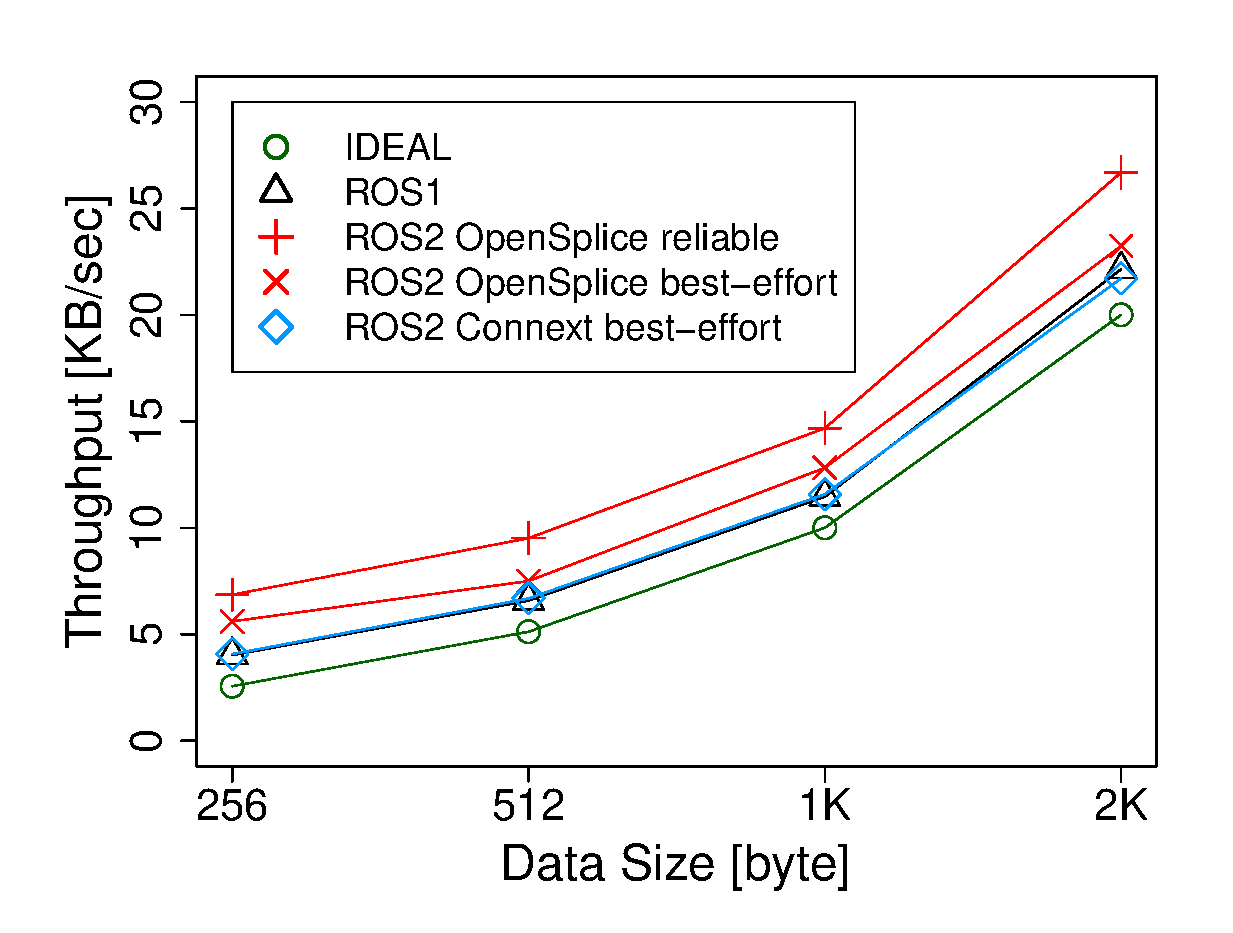
\includegraphics[width=1.0\linewidth]{../../figure/throughput_remote_small-data.eps}
        \caption{(1-a) and (2-b) \texttt{remote} cases throughput with small data}
        \label{fig:throughput_small}
      \end{minipage}
      &
      \begin{minipage}[t]{0.5\textwidth}
        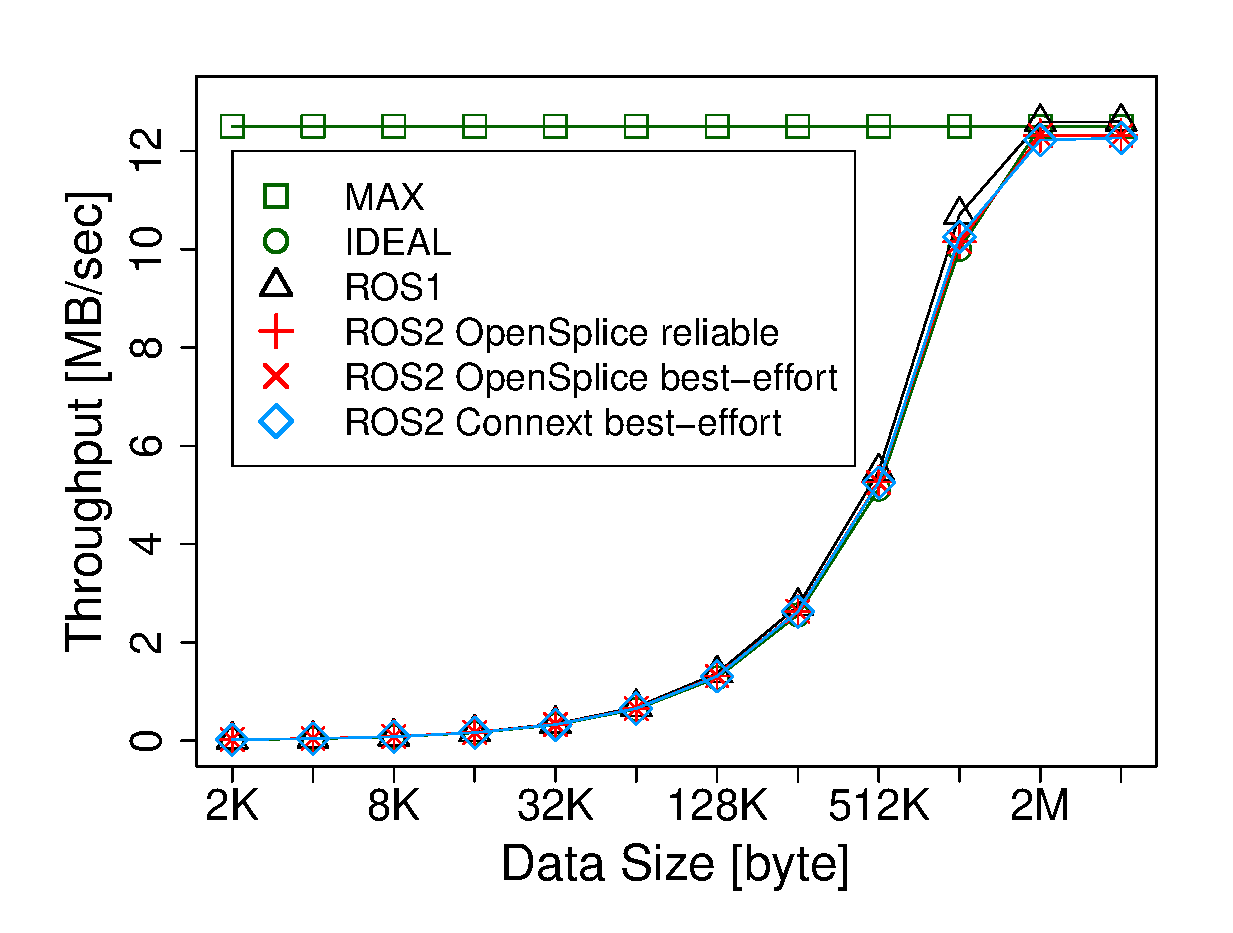
\includegraphics[width=1.0\linewidth]{../../figure/throughput_remote_large-data.eps}
        \caption{(1-a) and (2-b) \texttt{remote} cases throughput with large data}
        \label{fig:throughput_large}
      \end{minipage}
    \end{tabular}
  \end{figure*}

\end{enumerate}

\subsection{Unclear contributions}
\begin{enumerate}

\item \begin{flushleft}
    \textbf{Comment:}
  \end{flushleft}
  The contributions of the paper are essentially experimental results, but these results themselves are not sufficient. The authors do not provide any guidelines, lessons learned, or insight that they gained from their experiments.  Some examples of interesting questions to be answered from the data collected by the authors include:

  \begin{flushleft}
    \textbf{Our reply:}
  \end{flushleft}
  Thank you very much for pointing out our insufficient contribution and suggesting a lot of hint for lessons.
  To reply this comment and answer following interesting questions, we create ``Lessons Learned'' section.
  In this section, we show guidelines for ROS users to highlight our contributions from experiments in this paper.
  For precise sentences, please go on reading following our replies and revised paper.
  We hope you will be satisfied with our replies.

\item \begin{flushleft}
    \textbf{Comment:}
  \end{flushleft}
  Should ROS1 ever be used over ROS2, or do the benefits of ROS2 outweigh the costs?

  \begin{flushleft}
    \textbf{Our reply:}
  \end{flushleft}
  Thank you for suggesting a good question.
  ROS1 has relatively small latency and overhead throughput and rich packages and tools.
  ROS2 is under development and does not abstract some DDS APIs and QoS Policies.
  However, ROS2 some \emph{QoS Policies} and does not need master-node.
  This is important in terms of fault tolerance.
  Moreover, ROS2 will support RTOS and light DDS implementation for real-time embedded systems.
  We consider these benefits outweigh the cost and recommend the both with ros\_bridge.
  We have added sentences about this in ``Lessons Learned'' section to answer your comment.
  \begin{itembox}[|]{Added sentences about benefit of ROS2 in ``Lessons Learned'' section}
    Although ROS1 is low end-to-end latency and low throughput for pub/sub transport, ROS2 supports real-time embedded systems.
    To target these systems, it is inevitable that ROS1 users accept another approach.
    We consider ROS2 outweigh its cost for using DDS.
    Fault tolerance of ROS2 is superior because it is able to save past data with \emph{QoS Policy} and does not have a master \emph{node}.
    ROS2 will expand the scope of supported \emph{QoS Policies} for real-time systems.
    In addition, ROS2 is able to run on multiple platforms include RTOS and switch DDS implementation as needed.
  \end{itembox}\\
  \begin{itembox}[|]{Added sentences about collaboration in ``Lessons Learned'' section}
    At present, we should collaborate ROS1 and ROS2 with \texttt{ros\_bridge}.
    ROS2 has above goodness but it is under development.
    In addition, a lot of existing packages of ROS1 is useful for developers.
    While we develop a critical part of a application on ROS2, we implement other part on ROS1 with its rich packages and tools.
    We must be careful to reduce shared \emph{topics} and its data size because \emph{topics} conversion by \texttt{ros\_bridge} takes much time as shown in Figures \ref{fig;local_plot} and \ref{fig;local_small_plot}.
    When \emph{topic} communication between ROS1 and ROS2 is conducted in \texttt{remote} case, overhead latency is relatively small in Figures \ref{fig:remote_local_small_plot} and \ref{fig:remote_local_plot}.
  \end{itembox}\\

\item \begin{flushleft}
    \textbf{Comment:}
  \end{flushleft}
  What underlying implementation of DDS should people use, and why, or under what circumstances would one be better than the other? 

  \begin{flushleft}
    \textbf{Our reply:}
  \end{flushleft}
  Thank you for suggesting a good question.
  We recommend each DDS implementation depending on circumstances.
  In local case, OpenSplice is superior to others due to its capability and low latency caused by many threads.
  In remote case, Connext is superior because difference of latency is relatively small and we must consider bandwidth.
  Connext's throughput is minimum as shown in Figure ?.
  For embedded systems, in terms of memory and thread, we consider that FastRTPS is suitable from Tables ? and ?.
  We have added theses guidelines in ``Lessons Learned'' section to answer this question.
  \begin{itembox}[|]{Added sentences about ROS2 guideline in ``Lessons Learned'' section}
    We can get insight and guidelines for using ROS2 from these results.
    ROS2 supports \emph{QoS Policy} but there is trade-off of end-to-end latency and throughput.
    In \texttt{local} case, overhead latency of ROS2 is not trivial.
    From Section \ref{sec:latency}, the latency is caused by two data conversion for DDS and slower DDS transaction than ROS1.
    DDS end-to-end latency is constant until \emph{message} data size is lower than maximum packet size (64 KB) as shonw in \ref{fig:local_small_plot}.
    On the other hand, as one large \emph{message} is divided into several packets, the latency sharply increases as shonw in \ref{fig:local_plot}.
    Whether \emph{message} data size is over 64 KB or not is important issue especially in ROS2.
    While ROS2 has overhead latency, OpenSplice utilizes a lot of threads and processes faster than Connext as shown in Figures \ref{fig:dds_boxplot}.
    This is a reason why we currently should use OpenSplice in underlying implementation of DDS in \texttt{local} case.
    In \texttt{remote} case, although overhead latency is trivial, we must consider throughput for bandwidth.
    As shown in \ref{fig:throughput_small}, Connext is superior to OpenSplice in terms of throughput.
    This constant overhead throughput is predictable and exists no matter how small \emph{message} data size is.
    It influences especially when many kinds of topic are used with high Hz.
    We recommend Connext to consider minimum necessary throughput in \texttt{remote} case.
  \end{itembox}\\

\item \begin{flushleft}
    \textbf{Comment:}
  \end{flushleft}
  What can be done to improve the performance of the interface between ROS2 and DDS, or within the DDS implementations themselves?

  \begin{flushleft}
    \textbf{Our reply:}
  \end{flushleft}
  Thank you for your thoughtful comment.
  First, ROS2 must expand the scope of supposed QoS Policies for real-time system.
  It is a very important issue for real-time guarantee.
  Current QoS Policy is insufficient.
  Second, ROS2 should abstract alternative API such as asynchronous publisher and flow controller for large data transport.
  This improves DDS performance and reduce overhead latency.
  Finally, there are numerous DDS and vendor specific configuration options which might affect its performance.
  Tuning these configures for ROS2 is to do in order to improve performance within each DDS implementation.
  We have added some sentences to clarify above things as followed.
  \begin{itembox}[|]{Added sentences about alternative API in ``Lessons Learned'' section}
    We also clarify a need of alternative API for large \emph{message} to manga divided packets.
    It is critical to handle lager message.
    Abstraction of this shortens DDS end-to-end latency and fulfill deficiency of Table \ref{tb:capabilities}.
  \end{itembox}\\
  \begin{itembox}[|]{Added sentences about improvement of ROS2 in ``5. CONCLUSION'' section}
    Since ROS2 is under development, we must maximize DDS potential by tuning and abstracting more \emph{QoS Policies} and DDS configurations.
  \end{itembox}\\

\item \begin{flushleft}
    \textbf{Comment:}
  \end{flushleft}
  How does the switch to DDS from pure TCP or UDP protocols affect other performance factors in ROS2 systems? 

  \begin{flushleft}
    \textbf{Our reply:}
  \end{flushleft}
  Thank you for your suggestion.
  Before revision, we only indicate end-to-end latency affected by DDS.
  After revision, we show other performance factors by variable aspects.
  One additional factor is throughput in ``3.4 Throughput of ROS1 and ROS2'' section.
  We discuss throughput affected by DDS in this added section and clarify overhead throughput of each DDS implementations.
  Another factor is thread in ``'' section.
  The number of used threads are compared depending on DDS implementations.

\end{enumerate}

\subsection{Minor points}
\begin{itemize}

\item \begin{flushleft}
    \textbf{Comment:} Table 4 - ROS1 experiment says 2c, should be 1c
  \end{flushleft}

  \begin{flushleft}
    \textbf{Our reply:} Thank you very much for your careful reading. We have exchanged ``2c'' and ``1c''. (page 3)
  \end{flushleft}

\item \begin{flushleft}
    \textbf{Comment:} 3.3.1 ROS1 and ROS2 is much less than the difference between remote and local cases
  \end{flushleft}

  \begin{flushleft}
    \textbf{Our reply:} Thank you for pointing out our illegible expression. We have removed ``The difference in end-to-end latencies between'' and modified the sentence as you proposed. (in section 3.3.1)
  \end{flushleft}

\item \begin{flushleft}
    \textbf{Comment:} 3.3.2 with large data, ROS2 has significant overhead depending on the size of data
  \end{flushleft}

  \begin{flushleft}
    \textbf{Our reply:} Thank you for pointing out our unreadable expression. We have changed ``Compared to ROS1, with'' to ``With''. (in Section 3.3.2)
  \end{flushleft}

\item \begin{flushleft}
    \textbf{Comment:} Figure 12 and 13, invert legend
  \end{flushleft}

  \begin{flushleft}
    \textbf{Our reply:} Thank you for your suggestion. We have inverted the legends of Figure 12 and 13 for easy distinguishable difference. (in Section 3.3)
  \end{flushleft}

\item \begin{flushleft}
    \textbf{Comment:} Table 5 legend missing
  \end{flushleft}

  \begin{flushleft}
    \textbf{Our reply:} Thank you for pointing out our wrong part. We have fulfilled Tabel 5 legend as ``Comparison of ROS2 to Related Work''. (in Section 4)
  \end{flushleft}

\item \begin{flushleft}
    \textbf{Comment:} The authors use several implementations of DDS but it is unclear from their figures, which data is for OpenSplice, Connext or FastRTPS
  \end{flushleft}

  \begin{flushleft}
    \textbf{Our reply:} I'm sorry to provide unclear figures. We have added explanations for Figures 8, 9, 10, and 11 to clarify what DDS implementation we used. (in Section 3.3)
  \end{flushleft}

\item \begin{flushleft}
    \textbf{Comment:} Section 3.3.3 analyses performance for the two DDS frameworks with an explicit assumption regarding the performance of Opensplice vortex. The authors assume that the performance of Opensplice vortex professional edition is the same as the performance of Connext professional edition, but conduct their experiments only with the community edition of Opensplice. For a fair analysis, either the professional or community version should be used for both frameworks.
  \end{flushleft}

  \begin{flushleft}
    \textbf{Our reply:} Thank you for pointing out our unfair evaluations. 
    We tried building ROS2 with Vortex OpenSplice, but we could not succeed. 
    Currently, ROS2 does not support OpenSplice Professional Edition. For clear discussion, we added sentence ``,but ROS2 does not support this'' (``this'' means Vortex OpenSplice) in a footnote. (page 2) 
    In addition, after a evaluation of threads, we have changed our view that the performance of Opensplice vortex professional edition is the same as the performance of Connext professional edition. 
    Using OpenSplice, ROS2 has many threads (about 49 threads). 
    Parallelized procession by a lot of threads causes low latency and we assume that Vortex OpenSplice is faster than Connext.
  \end{flushleft}
  \begin{itembox}[|]{Added footnote in page 5}
    Vortex OpenSplice \cite{ospl_vortex}, i.e., OpenSplice commercial edition, supports shared memory transport \textcolor{red}{, but ROS2 does not supports this}. In this paper, OpenSplice DDS Community Edition is used because it is open-source.
  \end{itembox}\\

\end{itemize}

\newpage

\section{Response to 2\nd reviewer}
\begin{enumerate}

\item \begin{flushleft}
    \textbf{Comment:}
  \end{flushleft}
  The experiments provide good data, but unfortunately the data come only from a high-performance, multi-core system. 
  It will be useful to discuss performance in an embedded device used in robotics with some resource constraints.

  \begin{flushleft}
    \textbf{Our reply:}
  \end{flushleft}

\item \begin{flushleft}
    \textbf{Comment:}
  \end{flushleft}
  Since the comparison provides evaluations of ROS middleware replacements, considering alternatives (primarily ZMQ + Protobuf) would have made for a compelling case (for or against) the selected DDS approach.

  \begin{flushleft}
    \textbf{Our reply:}
  \end{flushleft}
  Thank you very much for your good insight. 
  Although these alternatives such as ZMQ + Protobuf should be evaluated, ROS2 firstly accepts DDS approach and only supports several DDS implementations. 
  To highlight this fact, we have added ``Currently ROS2 only supports some DDS implementations.''. (page 1) 
  Since ROS2 currently does not support ZMQ+Protobuf, this paper focuses evaluation of DDS approach to ROS and conducts its proof of concept.

\item \begin{flushleft}
    \textbf{Comment:}
  \end{flushleft}
  Additionally, further evaluations of the QoS policies would have been beneficial, since 100 ms deadline is rather meaningless for the message sizes, processor speeds, and network capacities used in the experimental evaluation.

  \begin{flushleft}
    \textbf{Our reply:}
  \end{flushleft}

\item \begin{flushleft}
    \textbf{Comment:}
  \end{flushleft}
  Finally, evaluation of performance of the middleware options under more constrained network resources would have been beneficial as well.

  \begin{flushleft}
    \textbf{Our reply:}
  \end{flushleft}

\end{enumerate}

\newpage

\section{Response to 3\rd reviewer}
\begin{enumerate}

\item \begin{flushleft}
    \textbf{Comment:}
  \end{flushleft}
  Despite this, the title and contributions are not clear, particularly, performance is a broad term and the authors mostly present results on message transmission. 
  The contribution should be stated more explicitly.
  While it is true that other practical considerations are explained, they are not properly highlighted.

  \begin{flushleft}
    \textbf{Our reply:}
  \end{flushleft}
  Thank you very much for your critical comment.
  To expand the scope of experiments, we have conducted additional evaluations.
  One is measurement of throughput in ``3.4 Throughput of ROS1 and ROS2'' section.
  Another is measurements of threads in ``'' section.
  The other is shared object memory in ``'' section.
  We consider that these broad evaluations and analysis represent the performance of ROS2 after revision.
  In addition, we have created new section ``Lessons Learned'' to clarify our contributions and practical considerations.
  In this section, we explicitly show guidelines for ROS users and highlight our contributions from experiments in this paper.
  This lessons will variable and should be shared among ROS users.
  
  For precise description of each section, please check our revised paper.
  
\item \begin{flushleft}
    \textbf{Comment:}
  \end{flushleft}
  One of the most promising improvements of ROS2 wrt ROS is the lack of a single point of failure (master). This should probably be highlighted!

  \begin{flushleft}
    \textbf{Our reply:}
  \end{flushleft}
  Thank you very much for pointing out a vital issue.
  This is important for fault tolerance and significant benefit of using ROS2.
  To highlight this point, we have added several sentences.
  \begin{itembox}[|]{Added sentences in ``2.1 Robot Operating System (ROS)'' section}
    In addition, due to use of DDS, ROS2 does not need a master process.
    \textcolor{red}{This is a import point in terms of fault tolerance.}
  \end{itembox}\\
  \begin{itembox}[|]{Added sentences in ``Lesson Learned'' section}
    We consider ROS2 outweigh its cost for using DDS.
    Fault tolerance of ROS2 is superior because it is able to save past data with \emph{QoS Policy} and does not have a master \emph{node}.
  \end{itembox}\\
  
\item \begin{flushleft}
    \textbf{Comment:}
  \end{flushleft}
  How exactly are the end-to-end delays (one way transmission) measured by the same computer? Please explain the process.

  \begin{flushleft}
    \textbf{Our reply:}
  \end{flushleft}
  
\item \begin{flushleft}
    \textbf{Comment:}
  \end{flushleft}
  In table 4: Why is there 'none' in the ROS2 best effort policy? Since there is no backlog saved on the nodes, all late joining nodes will suffer from the same problem as ROS nodes.

  \begin{flushleft}
    \textbf{Our reply:}
  \end{flushleft}
  Thank you for pointing out our lack of explanation.
  In best-effort policy, ``none'' means there is no inital loss when a subscriber-node is launched before a publisher-node begins to send messages.
  As you explained, a node with best-effort policy does not have backlog and there will be a lot of messag loss for lata-joining nodes.
  In Table 3, ``Inital loss'' means whether there is message loss or not for pre-joining nodes.
  ``Inital loss'' in not for late-joining nodes.
  After receiving your comment, we have modified sentences in the beginning of ``Capabilities of ROS1 and ROS2'' section to make it easy to understand.
  \begin{itembox}[|]{Added a sentence in ``Capabilities of ROS1 and ROS2'' section}
    In \texttt{best-effort policy}, a \texttt{subscriber-node} must be launched before a \emph{publisher-node} begins to send \emph{messages} for ``Initial loss'' none.
  \end{itembox}\\

\item \begin{flushleft}
    \textbf{Comment:}
  \end{flushleft}
  A major feature of ROS2, is to give Real Time guarantees on message deliveries, however, this is not compared. Specifically, when message loads are increased, a comparison would be welcomed.

  \begin{flushleft}
    \textbf{Our reply:}
  \end{flushleft}

\item \begin{flushleft}
    \textbf{Comment:}
  \end{flushleft}
  The authors say that Connext and OpenSplice maximum payload size is 64kB, but this is also the maximum payload of both TCP and UDP messages. Why is this an advantage/disadvantages of this?

  \begin{flushleft}
    \textbf{Our reply:}
  \end{flushleft}
  Thank you very much for indicating our unclear explanation.
  Connext and OpenSplice maximum payload size is officially described as 64KB in [http://www.prismtech.com/vortex/vortex-opensplice/performance] and [http://www.rti.com/products/dds/benchmarks.html].
  As a reviwer comments, it is also the maximum payload of IP packet.
  In DDS, message packet is sent following QoS.
  Hence, when large message is divided into several packets, DDS takes more time to manage these packets.
  There is some cases alternative API is needed 
  As shown in Figures 11, DDS highly depends on number of packets.
  According to these result, in terms of latency, we must be careful ...

\item \begin{flushleft}
    \textbf{Comment:}
  \end{flushleft}
  There is no mention whatsoever on which type of network is used to comunicate between two different machines. Is it a full-duplex ethernet connection, an unreliable WiFi connection, or some other network?
  This is important, since authors claim "Some failures with the best-effort policy are due to frequent message losses caused by non-reliable communications", which is dependent on the actual protocol.

  \begin{flushleft}
    \textbf{Our reply:}
  \end{flushleft}
  Thank you for pointing out import issue. 
  We have conducted \texttt{remote} case experiments with Full-Duplex 100BASE-TX 100Mbps Ethernet connection.
  Two machines are physically connected by LAN cable with a switcher.
  Thus, message loss occurs by UDP and not by network.
  To clarify this fact, we add network protocol in Table 2: ``Evaluation Environment''.
  \setcounter{table}{1}
  \begin{table*}[H]
    \caption{Evaluation Environment} 
    \centering
    \begin{threeparttable}
      \renewcommand{\arraystretch}{1.0}
      \label{tb:environment}
      \small
      \tabcolsep = 1.5mm              % side-margin in column
      \begin{tabular}{c|c||c|c}
        \hline
        \multicolumn{2}{c||}{ } & \textbf{\texttt{Machine1}} & \textbf{\texttt{Machine2}} \\ \hline \hline
        \multirow{4}{*}{CPU}   & Model number & Intel Core i5 3470 & Intel Core i5 2320 \\ 
        & Frequency & 3.2 GHz & 3.00 GHz \\ 
        & Cores & 4 & 4 \\ 
        & Threads & 4 & 4 \\ \hline
        \multicolumn{2}{c||}{Memory} & 16 GB & 8 GB \\ \hline 
        \multicolumn{2}{c||}{\textcolor{red}{Network}} & \multicolumn{2}{c}{\textcolor{red}{100 Mbps Ethernet / Full-Duplex}} \\ \hline
        \multicolumn{2}{c||}{ROS1} & \multicolumn{2}{c}{Indigo} \\ 
        \multicolumn{2}{c||}{ROS2} & \multicolumn{2}{c}{Cement (alpha3)} \\ 
        \multicolumn{2}{c||}{DDS implementations} & \multicolumn{2}{c}{Connext\tnote{1} / OpenSplice\tnote{2} / FastRTPS } \\ \hline 
        \multirow{2}{*}{OS} & Distribution & \multicolumn{2}{c}{Ubuntu 14.04} \\ 
        & Kernel & \multicolumn{2}{c}{Linux 3.13.0} \\ \hline
      \end{tabular}
      \begin{tablenotes}
      \item[1] RTI Connext DDS Professional \cite{rti_connext}
      \item[2] OpenSplice DDS Community Edition \cite{ospl_dds_community}
      \end{tablenotes}
    \end{threeparttable}
  \end{table*}
  
\item \begin{flushleft}
    \textbf{Comment:}
  \end{flushleft}
  What was the message set in each experiment? Only one message per experiment? Or was there any combination of messages in each experiment? If so, the scheduling algorithm should have been explained and the interference analysed.

  \begin{flushleft}
    \textbf{Our reply:}
  \end{flushleft}


\item \begin{flushleft}
    \textbf{Comment:}
  \end{flushleft}
  Missing results: Much of the information shared in robots is destined to multiple destinations. A possible improvement (maybe for future work) would be a comparison wrt multi-destination message distribution.

  \begin{flushleft}
    \textbf{Our reply:}
  \end{flushleft}

\end{enumerate}

\newpage


\section{Our modifications}

\begin{flushleft}
  \textbf{Comment:}
\end{flushleft}

\begin{flushleft}
  \textbf{Our reply:}
\end{flushleft}

\begin{itemize}
\item 
\item
\end{itemize}


\end{document}

